\section{Software} \label{sec:software} 

This section starts with a justification of why we choose Julia to 
implement the GSVD algorithm described in section \ref{alg}. 
Then we discuss the design of the interface, and implementation details. 
Finally, we list the GSVD available in other 
programming languages. 

\subsection{Why Julia}

\paragraph{Two-language problem.}

Julia is a new programming language that aims to address 
the so-called ``two-language problem'',  which designers 
and software developers need to face: they have to make a trade-off 
when designing or choosing a language -- it can either be relatively 
easy for humans to write as a dynamic language, or relatively easy for 
computers to run as a statically-typed language, 
but not both \cite{perkel2019julia}.

When it comes to the realm of numerical and scientific computing, 
the first language Fortran \cite{10.5555/541529} 
dated back to 1957. Over six decades, on one hand,
the landscape of computing has changed dramatically due to the 
advance of hardware, algorithms, and tremendous increased amount of data, 
among others. On the other hand, an unfortunate outcome is that the most challenging areas 
of scientific computing have benefited the least from the enhanced 
abstraction and productivity offered by higher-level languages. 
Modern scientific computing environments such as 
Python (Numpy)~\cite{van2011numpy}, 
R~\cite{ihaka1996r}, 
Mathematica~\cite{math}, and 
MATLAB~\cite{MATLAB}, to name a few, 
have grown in popularity among researchers and scientists of various disciplines, 
all of which are weakly or dynamically typed. 
Still, when it comes to performance, none of these favored languages 
can compete against Fortran and C for solving computationally intensive problems
because weakly or dynamically typed language needs type check for variables, statement, field,
and even object and class hierarchy at runtime \cite{bezanson2017julia}. 

\paragraph{Julia -- introduction.} 
As a dynamic language, Julia allows programmers to write high-level, generic and 
abstract code that closely resembles mathematical formulas 
\cite{bezanson2017julia, edelman2019julia}.
By making use of the following techniques, Julia can generate optimized native code for multiple architectures 
and can approach the speed of Fortran and C. \cite{Sengupta2019}
	\begin{itemize}
		\item Multiple dispatch using type system to select implementations: 
		
		``Multiple'' means that a function can have multiple implementations, called methods, distinguished by the type annotations added to parameters of the function. ``Dispatch'' means that at run-time, a function call is dispatched to the most specific method applicable to the types of the arguments.
		\item Code specialization against run-time types
		\item JIT (Just-In-Time) compilation using the LLVM compiler framework
	\end{itemize}


\paragraph{Julia -- features that we're particularly interested in.} ~ 
\begin{enumerate} 
\item {\bf A powerful approach to linear algebra.}

Vectors and matrices in Julia are based on and can be extended from the {\tt Array} type. 
While in C++ and Python matrices are stored in a row-first manner, they are stored in column-major in Julia, like Fortran. Elementary operations such as addition, subtraction, and multiplication are built-in in Julia.
Julia also provides native implementations 
for many common linear algebra operations in the \texttt{LinearAlgebra} library. 
Basic matrix operations are implemented with calls to 
BLAS and LAPACK routines; the default implementation is OpenBLAS. 
\begin{itemize} 
    \item Elementary operations:
    
    \begin{itemize}
    	\item Julia features component-wise operations. For example, component-wise multiplication writes as `{\tt .*}'. If {\tt f} is a function defined for single arguments and {\tt A} is a matrix, then {\tt f.(A)} is the matrix that results from component-wise operation of {\tt f} to the entries of {\tt A}. This is also known as broadcasting.

		\item Julia also offers matrix division from left {\tt B\textbackslash A} and right {\tt A/B}, which is equvivalent to computing $B^{-1}A$ and $AB^{-1}$ respectively. 
    
    \end{itemize}
    
    \item 
    LAPACK wrappers are implemented fully in Julia code, using \texttt{ccall} \textemdash{} calling C and Fortran code, without any ``glue'' code, code generation, or compilation. 
    All LAPACK routines are available in Julia. Julia users can write user-extensible wrappers 
    for BLAS and LAPACK on top of the \texttt{LinearAlgebra} library \cite{bezanson2017julia}. For instance, LAPACK provides BLAS-1 routine {\tt ddot} for computing the dot product of two vectors of double precision floating point type. This is already implemented in Julia as one method under the `{\tt *}' operation family. Still, we can write {\tt ddot} wrapper purely in Julia. Here's how it is implemented.  

% for indentation of code, verbatim requires space, not tab   
\begin{verbatim} 
    function compute_dot(DX::Vector{Float64}, DY::Vector{Float64})
        @assert length(DX) == length(DY)
        n = length(DX)
        incx = incy = 1
        product = ccall((:ddot_, "libLAPACK"),
                  Float64,
                  (Ref{Int32}, Ptr{Float64}, Ref{Int32}, 
                  Ptr{Float64}, Ref{Int32}),
                  n, DX, incx, DY, incy)
        return product
    end    
\end{verbatim}
	
	We declare the function with two arguments of {\tt Vector\{Float64\}} type and name it {\tt compute\_dot}. In this function, we first declare input arguments necessary to {\tt ddot}. Then we use {\tt ccall} to call LAPACK's {\tt ddot} routine. {\tt ccall} has four arguments:
	\begin{itemize}
		\item {\tt (:function\_name, "library\_name")} pair: in our example, {\tt (:ddot\_, "libLAPACK")}.
		\item return type of the function: {\tt Float64} in our example.
		\item a tuple of input types to the function in the library: in our example, {\tt (Ref\{Int32\}, Ptr\{Float64\}, Ref\{Int32\}, Ptr\{Float64\}, Ref\{Int32\})}.
		\item the actual argument values to be passed to the function: {\tt n, DX, incx, DY, incy} respectively in our example.
	\end{itemize} 
	Finally, we take the return value of {\tt ccall} as the return for the wrapper function. 
    
    \item 
    Matrices with special symmetries and structures arise often 
    in linear algebra and are frequently associated with various 
    matrix factorizations. Julia has a collection of special 
    matrix types. Table \ref{freq-mat} below summarizes the types of some special matrices that have been implemented in Julia. 
    
    \begin{table}[H]
    	\centering
    \begin{tabular}{|| c | c ||} \hline
    Type & Description \\ \hline\hline
    {\tt Symmetric}	& Symmetric matrix \\ \hline
    {\tt Hermitian}	& Hermitian matrix \\ \hline
    {\tt UpperTriangular} & Upper triangular matrix \\ \hline
    {\tt LowerTriangular} & Lower triangular matrix \\ \hline
    {\tt UpperHessenberg} & Upper Hessenberg matrix \\ \hline
    {\tt Tridiagonal} & Tridiagonal matrix \\ \hline
    {\tt SymTridiagonal} & Symmetric tridiagonal matrix \\ \hline
    {\tt Bidiagonal} & Upper/lower bidiagonal matrix \\ \hline
    {\tt Diagonal} & Diagonal matrix \\ \hline\hline
    \end{tabular}
	\caption{Commonly used special matrix types 
in Julia} \label{freq-mat}
	\end{table}
	
	Furthermore, Julia provides fast computation with specialized 
    routines that are specially developed for particular matrix types. 
    For example, for the SVD of a general dense matrix, Julia will use the default 
    SVD method {\tt svd!(A::StridedMatrix{T})}, which essential calls {\tt gesvd!} in LAPACK.
    The key part of the source code of this function is shown below.
    
    \begin{verbatim}
    function svd!(A::StridedMatrix{T}; full::Bool = false, 
    alg::Algorithm = default_svd_alg(A)) where T<:BlasFloat
        m,n = size(A)
        if m == 0 || n == 0
            u,s,vt = (Matrix{T}(I, m, full ? m : n), real(zeros(T,0)), 
                      Matrix{T}(I, n, n))
        else
            u,s,vt = _svd!(A,full,alg)
        end
        SVD(u,s,vt)
    end

    _svd!(A::StridedMatrix{T}, full::Bool, alg::DivideAndConquer) 
    where T<:BlasFloat = LAPACK.gesdd!(full ? 'A' : 'S', A)
    function _svd!(A::StridedMatrix{T}, full::Bool, alg::QRIteration) 
    where T<:BlasFloat
        c = full ? 'A' : 'S'
        u,s,vt = LAPACK.gesvd!(c, c, A)
    end
    \end{verbatim}
    
    On the contrary, if we want to compute the SVD of a bidiagonal matrix, Julia will use an optimzed 
    {\tt svd!(M::Bidiagonal\{<:BlasReal\})} instead. This function is a wrapper on top of LAPACK's {\tt bdsdc!} routine.
    We also show the key part of the source code of this function.
    
    \begin{verbatim}
    svdvals!(M::Bidiagonal{<:BlasReal}) = LAPACK.bdsdc!(M.uplo, 
                                          'N', M.dv, M.ev)[1]
    
    function svd!(M::Bidiagonal{<:BlasReal}; full::Bool = false)
        d, e, U, Vt, Q, iQ = LAPACK.bdsdc!(M.uplo, 'I', M.dv, M.ev)
        SVD(U, d, Vt)
    end
    \end{verbatim}
    
    \item
    Julia has support for sparse vectors and sparse matrices in the {\tt SparseArrays} module. In Julia, sparse matrices are stored in the Compressed Sparse Column (CSC) format. The CSC is represented as follows:
    \begin{verbatim}
    struct SparseMatrixCSC{Tv,Ti<:Integer} <: AbstractSparseMatrix{Tv,Ti}
        m::Int                  # Number of rows
        n::Int                  # Number of columns
        colptr::Vector{Ti}      # Column j is in colptr[j]:(colptr[j+1]-1)
        rowval::Vector{Ti}      # Row indices of stored values
        nzval::Vector{Tv}       # Stored values, typically nonzeros
    end
    \end{verbatim}
    Moreover, sparse matrix solvers call functions from SuiteSparse \cite{davis2015suitesparse}. Choleskey factorization, LU factorization and QR factorization of sparse matrices are now available. 

\end{itemize} 

\item {\bf Ease-of-use.} 

\begin{itemize} 
\item 
Julia is dynamically-typed, which means users need not worry about which types fit best in a given scenario.

\item 
Julia features garbage collection, thus memory management (allocation and destruction) will not be a manual effort, unlike in Fortran when we need to consider workspace requirement.

\item Generic, abstract, and extendible syntax by multiple dispatch

In Fortran, multiplication between two scalers, scaler and vector, matrix and vector, and two matrices have different method names. This is counter-intuitive to the abstraction of math: all of this operations are multiplication, why can't they share the same name? Fortunately, in Julia, with the help of multiple dispatch, which allows users to depart from the limitations of type-based designs, we can leverage the expressive power of generic functions. 
For instance, elementary operations like addition and multiplication in Julia are intuitive and generic, as simple as math, shown below in Table \ref{add-mul}. 

\begin{table}[H]
\centering
\begin{tabular}{|| c | c | c ||} \hline
Operator & Function & Operand \\ [0.5ex] \hline\hline
\texttt{+} & add numbers/vectors/matrices & 
\makecell{\texttt{Int, Float, Vector, }\\ 
\texttt{Abstract Matrix, Dense Matrix, $\cdots$}} \\ \hline
\texttt{*} & multiply scale or compose & \texttt{Number, Function} \\ 
\hline\hline
\end{tabular}
\caption{Generic commands of addition and multiplication of different types 
in Julia}
\label{add-mul}
\end{table}

Further, with multiple dispatch, users can extend the SVD family by implementing the SVD of other types, tensor, for instance. These new methods will have separate implementation, but share the same method name {\tt svd}.

\item
Julia is interactive with a full-featured interactive command-line REPL (read-eval-print loop) built into the Julia executable. It resembles to the interactive programming environment Python(IPython) and R(RStudio). In 2015, a web-based interactive computational platform Jupyter (named after Julia, Python and R) that spun off from IPython was launched.  

\item
Syntax similarity to MATLAB:

\begin{itemize}
\item 
Both Julia and MATLAB use $\texttt{end}$ keyword to 
indicate code block structure, e.g. loops, functions. 

\item 
In linear algebra, MATLAB programmers may find Julia more friendly because the array index 
in Julia also starts at 1, not 0. 

\item 
Table \ref{freq-decomp} below summarizes a list of Julia commands for frequently used 
matrix factorizations, and their counterparts in MATLAB. 

\begin{table}[H]
\centering
\scalebox{0.65}{
\begin{tabular}{|| c | c | c ||} \hline
Julia command & MATLAB command & Description \\ [0.5ex] \hline\hline
\texttt{schur(A::StridedMatrix) -> F::Schur} & \texttt{T = schur(A)} & Schur decomposition \\ \hline
         \texttt{lu(A, pivot=Val(true); check = true) -> F::LU} & \texttt{[L,U] = lu(A)} & LU decomposition \\ \hline
         \texttt{qr(A, pivot=Val(false)) -> F} & \texttt{[Q,R] = qr(A)} & QR decomposition \\ \hline
         \texttt{eigen(A; permute::Bool=true, scale::Bool=true, sortby) -> Eigen} & \texttt{[V,D] = eig(A)} & Eigenvalues and eigenvectors \\ \hline
         \texttt{svd(A; full::Bool = false) -> SVD} & \texttt{[U,S,V] = svd(A)} & Singular value decomposition \\
         \hline\hline
        \end{tabular}
}
\caption{Interfaces of commonly used matrix decompositions 
in Julia and MATLAB} \label{freq-decomp}
\end{table}
\end{itemize}

\end{itemize} 


\item {\bf Speed.}  

The core design decision, type inference through method specialization 
via multiple dispatch is what allows Julia to be very easy for 
a compiler to make into efficient code. 

\begin{itemize} 
\item Method specialization.
In short, method specialization is to run the right code at the right time. Julia’s compilation strategy is built on runtime type information. Every time a method is called with a new tuple of argument types, it is specialized to these types. Optimizing methods at invocation time, rather than ahead of time, provides the JIT with key pieces of information: the memory layout of all arguments is known, allowing for unboxing of objects and direct field access. Specialization, in turn, allows for devirtualization. Devirtualization replaces method dispatch with direct calls to a specialized method. This reduces dispatch overhead and enables inlining. The specialized method is added to the function’s dispatch table so that future calls with the same combination of argument types can reuse the generated code \cite{bezanson2018julia}.

\item Type inference.
Types of program expressions and variables are inferred by forward data-flow analysis \cite{bezanson2012julia}. Julia uses a set constraint-based analysis with constraints arising from return values, method dereferences, and argument types. Type requirements need to be satisfied at function call sites and field assignments. The system propagates constraints forward to satisfy requirements, inferring the types for intermediate values along the way.
\end{itemize} 

\end{enumerate} 

\subsection{Interfaces of GSVD in Julia}

The outputs of the GSVD algorithm consist of six matrices and two integers. 
To follow Julia's convention as an object-oriented language, we encapsulate 
all the outputs into a immutable composite type defined by {\tt struct} keyword,
followed by a block of field names, 
optionally annotated with types using the {\tt ::} operator.  In addition, {\tt <:} keyword 
connects a type with its supertype (``parent'') on the right hand side.
With composite type, users do not need to explicitly enumerate every matrix 
or integer in the return statement when they only want to access part of the outputs. 
We name the composite type {\tt GeneralizedSVD}. 

%\begin{lstlisting}[language=julia, style=jlcodestyle]
\begin{verbatim} 
    struct GeneralizedSVD{T} <: Factorization{T}
        U::AbstractMatrix{T}
        V::AbstractMatrix{T}
        Q::AbstractMatrix{T}
        C::AbstractMatrix{T}
        S::AbstractMatrix{T}
        k::Int
        l::Int
        R::AbstractMatrix{T}
    end
\end{verbatim} 
%\end{lstlisting}

Interfaces in Julia, particularly in ``\texttt{LinearAlgebra}'' library, 
are two-fold: one makes a copy of the input matrices or vectors, which
is convenient for testing purposes and is suitable for small inputs; 
the other one overwrites the inputs to save space and reduce communication overhead
between memory and cache. 

When designing the interface 
of the GSVD, we also take multiple dispatch into consideration. 
Multiple dispatch allows a function to be written 
generically and thus maintains the language's expressiveness.
It enables SVD of one matrix and GSVD of a matrix pair 
to share a single interface name, but with different number or types of 
arguments.  

\bigskip

Therefore, we provide two interfaces for the GSVD.  
%\begin{lstlisting}[language=julia, style=jlcodestyle]
\begin{verbatim} 
        svd(A, B) -> GeneralizedSVD
\end{verbatim} 
%\end{lstlisting}
or
%\begin{lstlisting}[language=julia, style=jlcodestyle]
\begin{verbatim} 
        svd!(A, B) -> GeneralizedSVD
\end{verbatim} 
%\end{lstlisting}

\paragraph{Common features of two interfaces.} 
Both interfaces compute the generalized SVD of \texttt{A} and \texttt{B},
returning a \texttt{GeneralizedSVD} object \texttt{F}, 
such that 
\begin{center} 
\texttt{A = F.U*F.C*F.R*F.Q'} 
\quad and \quad 
\texttt{B = F.V*F.S*F.R*F.Q'}. 
\end{center} 
For an \texttt{m}-by-\texttt{n} matrix \texttt{A} and \texttt{p}-by-\texttt{n} matrix \texttt{B},
\begin{itemize}
\item \texttt{U} is an \texttt{m}-by-\texttt{m} orthogonal matrix,
\item \texttt{V} is a \texttt{p}-by-\texttt{p} orthogonal matrix,
\item \texttt{Q} is an \texttt{n}-by-\texttt{n} orthogonal matrix,
\item \texttt{C} is an \texttt{m}-by-\texttt{(k+l)} diagonal matrix with 1s in the first \texttt{k} entries,
\item \texttt{S} is a \texttt{p}-by-\texttt{(k+l)} matrix whose top right \texttt{l}-by-\texttt{l} block is diagonal,
\item \texttt{R} is a \texttt{(k+l)}-by-\texttt{n} matrix whose rightmost \texttt{(k+l)}-by-\texttt{(k+l)} block is nonsingular upper block triangular,
\item \texttt{k+l} is the effective numerical 
rank of the matrix \texttt{[A; B]}. One can get {\tt k+l}
from {\tt F.k + F.l} 
\end{itemize}

\paragraph{Differences of two interfaces.}
After calling \texttt{svd(A, B)}, {\tt A} and {\tt B} will remain the same. By contrast,  
after calling \texttt{svd!(A, B)}, {\tt A} and {\tt B} will be overwritten. Specifically,
let $R$ be the {\tt R} matrix of the return object {\tt F},
\begin{enumerate}
	\item If $m-k-\ell \geq 0$
		\begin{equation*}
			R = \bordermatrix{ 
               & n-k-\ell & k + \ell \cr
    			\hfill k+\ell & 0 & R_{0} \cr}
		\end{equation*}
		$R_{0}$ is the same as \texttt{A[1:k+l,n-k-l+1:n]}.
	\item If $m-k-\ell <0$
		\begin{equation*}
			R = \bordermatrix{ 
               & n-k-\ell & k & m-k & k+\ell-m \cr
               \hfill k & 0 & R_{11} & R_{12} & R_{13} \cr
    			\hfill m-k & 0 & 0 & R_{22} & A_{23} \cr
    			\hfill k+\ell-m & 0 & 0 & 0 & R_{33} \cr}
		\end{equation*}
		$\begin{pmatrix}
			R_{11} & R_{12} & R_{13} \\
			0 & R_{22} & R_{23}
		\end{pmatrix}$
		is the same as \texttt{A[1:m, n-k-l+1:n]} and $R_{33}$ is equal to 
		\texttt{B[m-k+1:l,n+m-k-l+1:n]}.
\end{enumerate}


\subsection{GSVD module and implementation details}
\begin{enumerate} 
\item 
The structural unit called \texttt{module} is native in Julia to 
group relevant functions and definitions. We create two modules
for the GSVD algorithm. 

\item 
The main module of the GSVD algorithm is \texttt{GSVD}. In {\tt GSVD}
module, we first declare the composite type {\tt GeneralizedSVD}, create its constructor,
and a function for neat display.
This module also contains three functions below:
	\begin{itemize}
		\item {\tt svd}: main routine,
		\item {\tt preproc}: pre-processing subroutine,
		\item {\tt householderqr}: Householder QR decomposition subroutine.
	\end{itemize}
	
\item 
In addition, considering that the safe diagonalization not only serves 
as a building block for the GSVD algorithm, but is also a 
tool in other applications, we have separated the safe diagonalization 
as a stand alone module called \texttt{SafeDiag}. It contains routine {\tt safeDiag}.

\item 
The GSVD algorithm starts from the main function \texttt{svd} 
under module \texttt{GSVD}. It then calls \texttt{preproc}. 
Once return, it calls function \texttt{safeDiag} intermodularly. 
Finally, upon return, the main function post-processes to 
formulate the outputs. Figure \ref{seq_diag} shows the sequence of the major function 
calls.

 		\begin{figure}[H]
            \centering
              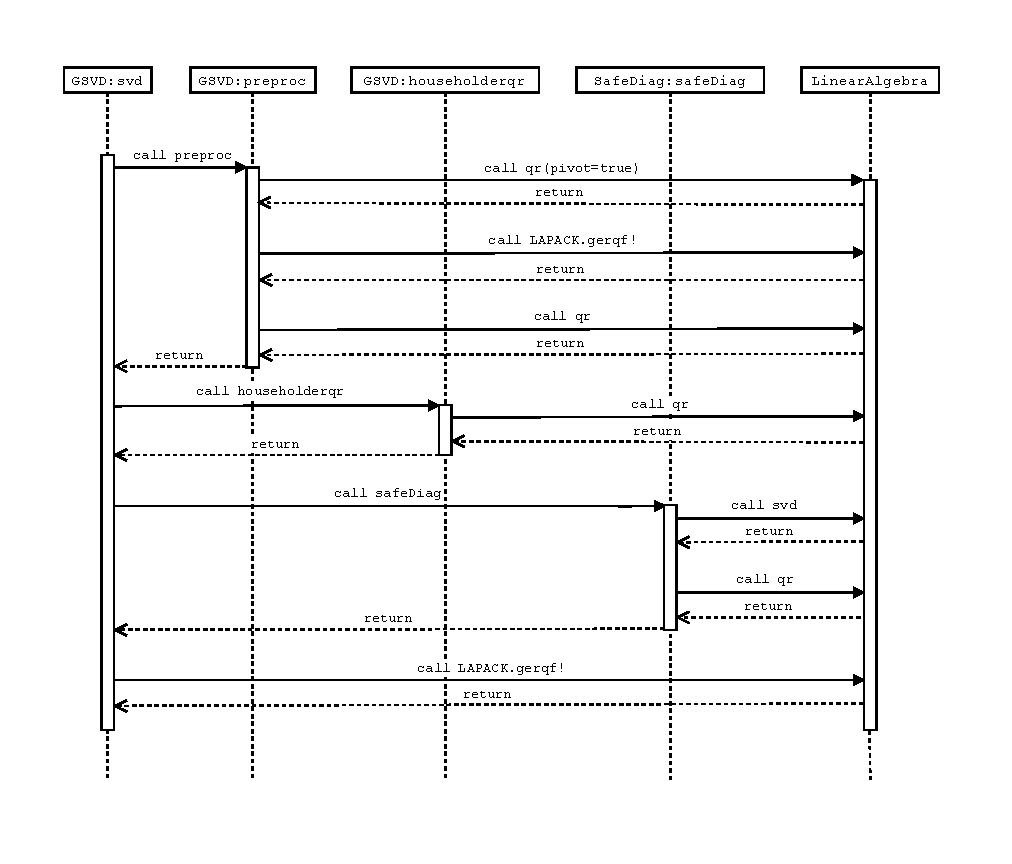
\includegraphics[width=\linewidth]{fig/gsvd_seq_diag.pdf}
              	\caption{Sequence diagram for the GSVD}
               \label{seq_diag}
        \end{figure} 


\item The details of each major functions are discussed below. 

\begin{itemize} 
\item \fbox{\texttt{GSVD:preproc}}

    This step is to reduce two input matrices $A$ and $B$ into two upper triangular forms. This is done via a call to \texttt{preproc}. This function makes use of three fundamental orthogonal decompositions. 
    \begin{enumerate}
    	\item First is QR decomposition with column pivoting to reveal the numerical rank of $B$ and $[A; B]$ without forming the matrix explicitly. This is done by a call to \texttt{qr(A, pivot=Val(true)))}. Let \texttt{tolB} as the tolerance to determine the effective rank of $B = \ell$.
		\begin{equation*}
			tol_{B} = max\{p, n\}\Vert B \Vert_1 \epsilon
		\end{equation*}
		where $\epsilon$ is the machine precision of \texttt{Float64}. \\
		We also use QR decomposition with column pivoting again on the leftmost $n-\ell$ columns of $A$. Similarly, by defining
		\begin{equation*}
			tol_{A} = max\{m, n\}\Vert A \Vert_1 \epsilon
		\end{equation*}
		we compute the effective rank of $[A; B] = k+ \ell$.
		\item Second is RQ decomposition of the top $\ell$ rows of $B$ if $n > \ell$ via a call to \texttt{LAPACK.gerqf!}. It is called a second time on $A$ if $n - \ell > k$.
		\item Third is QR decomposition of $A$ when $m > k$ by calling \texttt{qr}. 
	\end{enumerate}
	Upon return to \texttt{svd}, two of the upper triangular matrices overwrites $A$ and $B$, the orthogonal matrices are placed in U, V, and Q and rank information is stored in $k$ and $\ell$.

\item \fbox{\texttt{GSVD:householderqr}} 
    
    This step is to reduce two upper triangular matrices to one and is done by calling \texttt{householderqr}. On entry, two triangular matrices are stacked together and passed as the arguments of \texttt{qr}. On exit, $Q_1$ and $Q_2$ overwrites inputs.  
    
\item \fbox{\texttt{SafeDiag:safediag}}
    
    This step calls \texttt{safeDiag} from module \texttt{SafeDiag}. This function requires SVD, and QR decomposition. This is done by calls to \texttt{svd}, \texttt{qr} respectively. 
    \begin{enumerate}
    	\item We first compute SVD of $Q_{2}$. To preserve the order of $\{\cos\theta\}$, we have to reverse the order of the singular values of $Q_{2}$. 
		\item Since $\{\cos\theta\}$ are already sorted, we take advantage of binary search to find the threshold $r$.
		\item QR decomposition of the multiply of $Q_{1}$ and right singular vectors of $Q_{2}$. $R$ is not only triangular but diagonal. However, sanitization is necessary to assure the non-negativity of the diagonal entries. 
    \end{enumerate}
    
    It return $U_1, V_1, Z_1, C, S$ on exit.   

\item Post-processing:

    In this step, we update matrix $U$, $V$ and $Q$ by matrix-matrix multiply. To formulate $R$, we utilize RQ decomposition via a call to \texttt{LAPACK.gerqf!}. Finally, we put matrices $U, V, C, S, Q$ and $k$, $\ell$ into the constructor of \texttt{GeneralizedSVD} as return. 

\end{itemize}

\item We implement the GSVD algorithm in Julia 1.3 using \texttt{Float64} data. Our current implementation is able to be extended for {\tt Float32} type in the future. 

\end{enumerate} 


\subsection{Lessons and caveats} 
We capture some pitfalls that might be a bottleneck, 
and thus are worth mentioning.
\begin{itemize} 

\item {\bf Some inconsistent interface design.}

As a modern programming language, Julia supports multiple dispatch, that is, parametric polymorphism. A good example is that the GSVD interface reuses the name of the SVD of a single matrix $A$ by taking two matrices as arguments. Unfortunately, this principle is not fully implemented. For instance, when computing the matrix norm of {\tt [1 2 3; 4 5 6; 7 8 9]}, one may intuitively call \texttt{norm([1 2 3; 4 5 6; 7 8 9])}. However, this will not produce the desired result as shown below. What it actually computes is the 2-norm of the vector formed by iterating every entry of this matrix. Equivalently, it computes {\tt norm([1 2 3 4 5 6 7 8 9])}. To get the proper matrix norm, instead, one may want to use \texttt{opnorm([1 2 3; 4 5 6; 7 8 9])}. 

\begin{table}[H]
\centering
\begin{tabular}{|| c | c ||} \hline
Julia command/result & MATLAB command/result\\ [0.5ex] \hline\hline
\makecell{\texttt{norm([1 2 3; 4 5 6; 7 8 9])} \\
16.881943016134134} & \makecell{\texttt{norm([1 2 3;4 5 6;7 8 9])} \\ 16.8481} \\
\hline\hline
\makecell{\texttt{opnorm([1 2 3; 4 5 6; 7 8 9])} \\
16.84810335261421} & N/A \\
\hline\hline
\end{tabular}
\label{norm-api}
\end{table}

\item {Performance relies on ``proper'' implementation.}

Our GSVD algorithm involves many operations with subarrays and submatrices. Naturally, we would use {\tt [start\_i:end\_i,start\_j:end\_j]} to get a block matrix (slicing) from the entire matrix. However, in Julia, this could be a significant performance issue since slicing an array/matrix creates a copy of the selected subarray/submatrix, which is computational expensive. For instance, if we want to get the sum of subarray, we might do the following in Julia:  
%To make things worse, if a sliced matrix is passed as the return value, the result will be inaccurate as it is not overwritten in the original matrix. 
\begin{verbatim}
    x = rand(10^6);
    fcopy(x) = sum(x[2:end-1]);
    @time fcopy(x);
  	    0.003051 seconds (7 allocations: 7.630 MB)
\end{verbatim}

An alternative is to create a ``view'' of the array, which is an array object that actually references the data of the original array in-place, without making a copy. This can be done for individual slices by calling function \texttt{view}, or more simply for a whole expression or block of code by putting macro \texttt{@views} in front of that expression. This could improve the performance significantly. In the following code, we rewrite the function to calculate the sum of suarray with macro \texttt{@views}. One can tell that by doing so, the speedup is three-fold. 

%\begin{lstlisting}[language=julia, style=jlcodestyle]
\begin{verbatim}
    x = rand(10^6);
    @views fview(x) = sum(x[2:end-1]);
    @time fview(x);
        0.001020 seconds (6 allocations: 224 bytes)
\end{verbatim}
%\end{lstlisting}

\end{itemize} 

Many other features of Julian have not been studied and explored 
by the author, most notably, parallelism. This could be 
a good direction for future work. 


\subsection{GSVD in other languages}  
A number of numerical computing platforms feature 
the GSVD is listed in the following table. 
%Table \ref{tab:gsvdlang} is a list of ones we know of. 
    
%\begin{table}%[H]
%\centering
\begin{center} 
\scalebox{0.80}{
\begin{tabular}{|c|c|} \hline
Language & GSVD Documentation \\ \hline\hline
            Native Julia (proposed) &  \makecell[l]{\texttt{svd(A, B) -> GeneralizedSVD} \\ Computes the generalized SVD of \texttt{A} and \texttt{B},  returning a \texttt{GSVD} factorization\\ object \texttt{F}, such that \\ \texttt{A = F.U*F.C*F.R*F.Q'} and \texttt{B = F.V*F.S*F.R*F.Q'}.}\\ \hline
            Julia 1.3 (LAPACK wrapper) &  \makecell[l]{\texttt{svd(A, B) -> GeneralizedSVD} \\ Computes the generalized SVD of \texttt{A} and \texttt{B},  returning a \texttt{GeneralizedSVD}\\ factorization object \texttt{F}, such that \\ \texttt{A = F.U*F.D1*F.R0*F.Q'} and \texttt{B = F.V*F.D2*F.R0*F.Q'}.}\\ \hline
            MATLAB (2019b) & \makecell[l]{\texttt{[U,V,X,C,S] = gsvd(A,B)} \\
            Returns unitary matrices \texttt{U} and \texttt{V}, a (usually) square matrix \texttt{X}, and \\ nonnegative diagonal matrices \texttt{C} and \texttt{S} so that \\
                \texttt{A = U*C*X', B = V*S*X', C'*C + S'*S = I}.}\\ \hline
            Mathematica & \makecell[l]{\texttt{SingularValueDecomposition[{m,a}]} \\
            Gives a list of matrices \{\texttt{{u,ua},{w,wa},v}\} such that \texttt{m} can be written as \\ \texttt{u.w.Conjugate[Transpose[v]]} and \texttt{a} can be written as \\ \texttt{ua.wa.Conjugate[Transpose[v]]}. } \\ \hline
            R (geigen v2.3, LAPACK wrapper) & \makecell[l]{\texttt{z <- gsvd(A, B)}\\
            Computes The Generalized Singular Value Decomposition of matrices \\ $A$ and $B$ such that $A = UD_{1}[0 \ R]Q^{T}$ and $B = VD_{2}[0 R]Q^{T}$. Note that \\ the return value is the same as the output of LAPACK 3.6 and above. }
            \\\hline
            Python (R. Luo's thesis) &  \makecell[l]{Didn't disclose API design. The author defined GSVD as follows: \\
            Given two $M_i$-by-$N$ column-matched but row-independent matrices $D_{i}$, \\ each with full column rank and $N \leq Mi$, the GSVD is an exact \\ simultaneous factorization $Di = Ui \Sigma_i V^T, i = 1, 2$. $U_i$ is $M_i$-by-$N$ and \\ are column-wise orthonormal and $V$ is $N$-by-$N$ nonsingular matrix with\\ normalized rows. $diag(\Sigma_i)$ returns two lists of $N$ positive values and \\the ratios are called the generalized singular values.} \\ \hline
        \end{tabular}
} 
\end{center} 
% \caption{GSVD in different languages} \label{tab:gsvdlang}
%\end{table}
